\subsection{Design Overview of \gls{uefi}}
The UEFI construction is depending on the below listed primal elements:

\begin{itemize}
	\item \textbf{Re-utilizing of already existing interfaces} - In order to keep up assets in existing infrastructure  codebase, both at the OS and firmware level, many different existing specifications which are usually implemented on platforms harmonious with supported processor specifications has to be developed on platforms which is able to comply with specification of the UEFI.
	\item \textbf{System partition} characterizes a partition and file system which are to developed to grant safe sharing between various different vendors and various purposes. The power to include a disjoint, shareable system partition exists a chance to gain platform value-add without importantly thriving the need for nonvolatile memory of platform.
	\item \textbf{Boot services} are responsible to offer interfaces for devices and system functionality which could be utilized during the time of ongoing boot process. Device access is abstracted by \say{handles} and \say{protocols}. This features reuse the investment in already existing BIOS codebase by persisting underlying implementation necessity out of the specification without giving execution load to the consumer accessing device.
	\item \textbf{Runtime services} - A stripped set of runtime services is given to guarantee seize abstraction for resources of platform hardware which could be required by the OS while its conventional operations.
\end{itemize}

\begin{figure}[h]
	\centering
	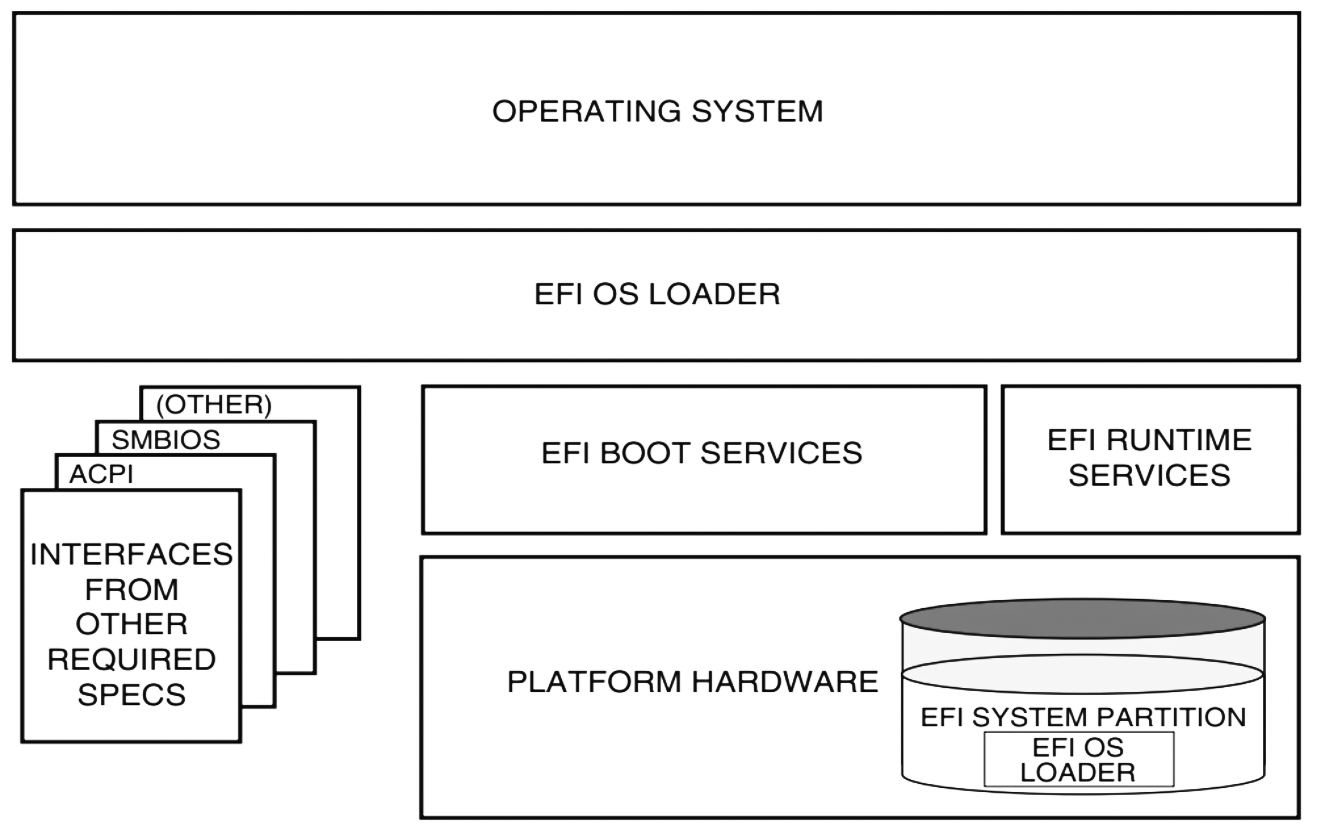
\includegraphics[width=0.8\linewidth]{design/uefi-conceptual-overview}
	\caption{UEFI Conceptual Overview}\label{fig:design-uefi-conceptual-overview}
\end{figure}

\textbf{Error! Reference source not found} determines the fundamental interaction of the different component parts of an UEFI specification-amenable system which are utilized to carry out platform and OS boot.

From the system partition, the os loader image is retrieves by the platform firmware. The specification supplies for a diversity of media and mass storage device types as \say{disk}, \say{CD-ROM}, and \say{DVD} as well as \say{remote boot} via a network (also known as LAN boot or network boot). By the use of extensible protocol interfaces, there is possibility to include many other boot media types but also these would need OS loader alteration if they need to use the protocols.

Once begun, the OS loader proceeds to boot the whole operating system. To achieve this it could utilize the EFI boot services and interfaces characterized by respected specifications to analyze, embrace, and initialize the several platform components and the OS software which controls them. Also, for the OS loader will be capable to access EFI runtime services while in boot phase.

\subsubsection{Goal of UEFI Driver}
Majorly below are the listed motives to be expected to achieve by the UEFI Driver:
\begin{itemize}
	\item \textbf{Compatible} - Any driver who conformist to the specification has to hold up compatibility along with the  UEFI and EFI Specification. Hence, the UEFI Driver Modal brings up benefits of the extensibility mechanisms in the UEFI Specification to include the desired and necessary features.
	\item \textbf{Simple} - Any driver who conformist to the specification has to be simpler to develop and maintain. The UEFI Driver Modal has to permit a driver writer to focus on the ad hoc device for which the driver is to be developed. A driver should not be related to issues correspondence to platform management or policy of platform. These circumstance should be left over for the system firmware.
	\item \textbf{Scalable} - The UEFI Driver Modal requires the adaptability for all kind of platforms including mobile, embedded systems, workstations, servers as well as desktop systems.
	\item \textbf{Flexibility} - The UEFI Driver Modal have to have capability to enumerate over every the devices (or only the relevant devices needed to boot the OS). With the minimum device enumeration support for fast boot ability can be achieved and the full device enumeration results to provide capability for performing system maintenance, or system diagnostics, OS installations on any boot device exists on the system.
	\item \textbf{Extensible} - The UEFI Driver Modal must be able to unfold to succeeding bus types as and when they are characterized.
	\item \textbf{Portability} - Every drivers transcribed in the UEFI Driver Model has to be portable among platforms and within every founded processor architectures.
	\item \textbf{Interoperability} -  Every drivers has to coexist along with every other firmware and drivers and also do so without incurring conflicts for any resource.
	\item \textbf{Describing hierarchies of complex bus} - The UEFI Driver Modal has to be capable to key out a all kind of bus topologies from the platforms as simple as single bus to platforms with extremely complex bus which may consists of multiple buses of different kind.
	\item \textbf{Address the issues for legacy ROM option} - The UEFI Driver Modal needs to instantly come up and resolve the restrictions and regulations of legacy ROM options. Especially, it has to be capable to build add-in device cards which supports both UEFI drivers and legacy ROM options. However, maintaining this backward compatibility, the solution with proposed methodology should also provide a way to migrate from legacy ROM option driver to UEFI driver.
\end{itemize}

\subsection{\gls{uefi}/\gls{pi} Firmware Images}
\gls{uefi} and \gls{pi} specifications characterize the standard format for EFI firmware storage devices which includes FLASH or any other nonvolatile storage which are separated in \say{Firmware Volumes}.
\begin{figure}[!htbp]
  \centering
  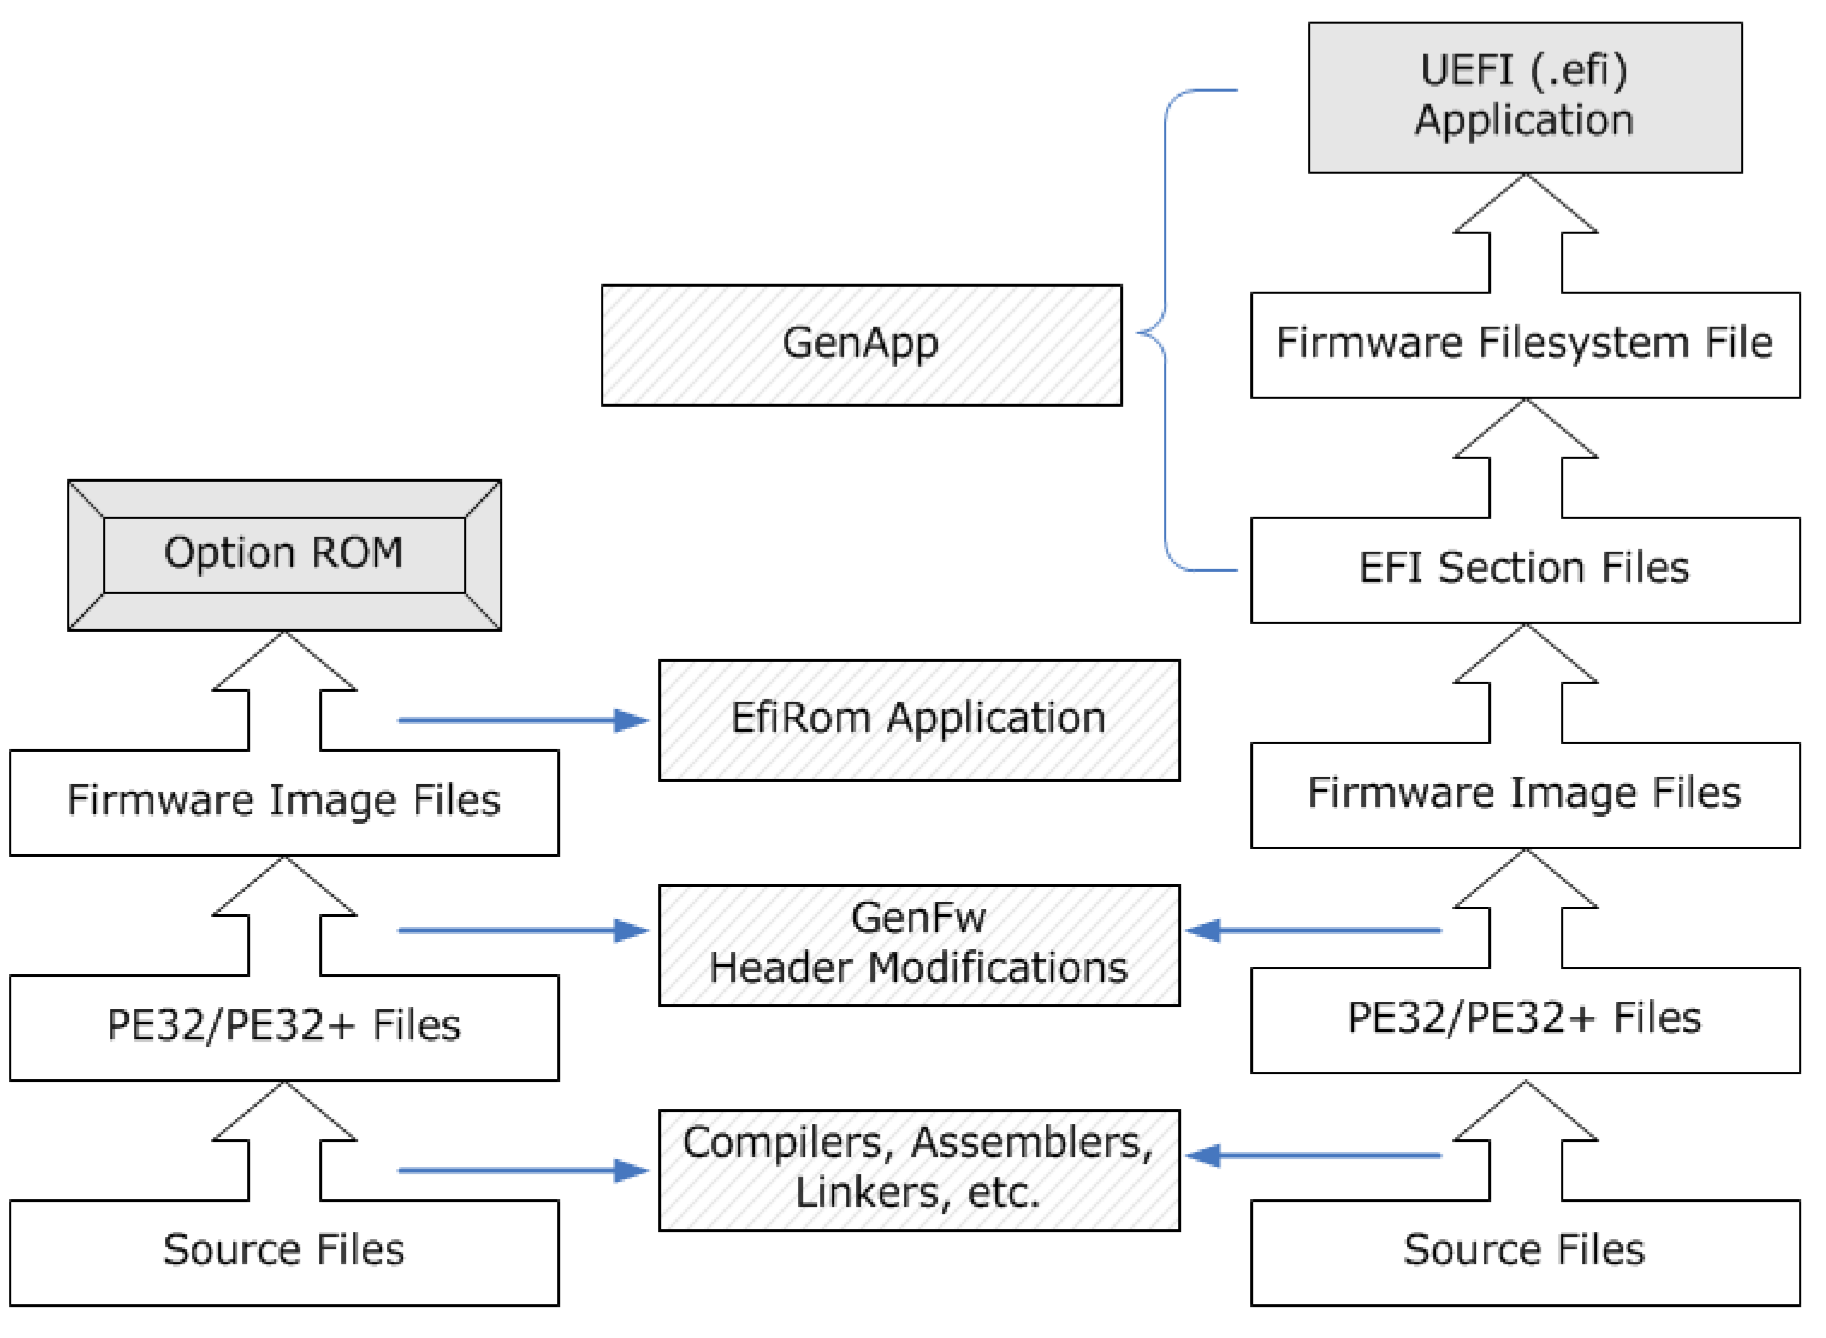
\includegraphics[width=0.9\linewidth]{design/efi-application-creation}
  \caption{UEFI/PI Firmware Image Creation}\label{fig:design-efi-application-creation}
\end{figure}

Build systems should have the capability of processing files to construct the file formats represented by the \gls{uefi} and PI specifications. The tools which are supplied as part of the \say{\gls{edk2} BaseTools package} processes files compiled via third party scripts and tools, as well as unicode files and text files in order to construct UEFI or PI amenable binary image file. In few cases, where UEFI or PI specifications don't have an corresponding file format for input such as the \say{Visual Forms Representation (VFR)} files utilized to make PI compliant IFR contents, scripts, tools and documentation have been supplied which permits the user to create text files that are treated into formats specified by UEFI or PI specifications.

\begin{figure}[!htbp]
  \centering
  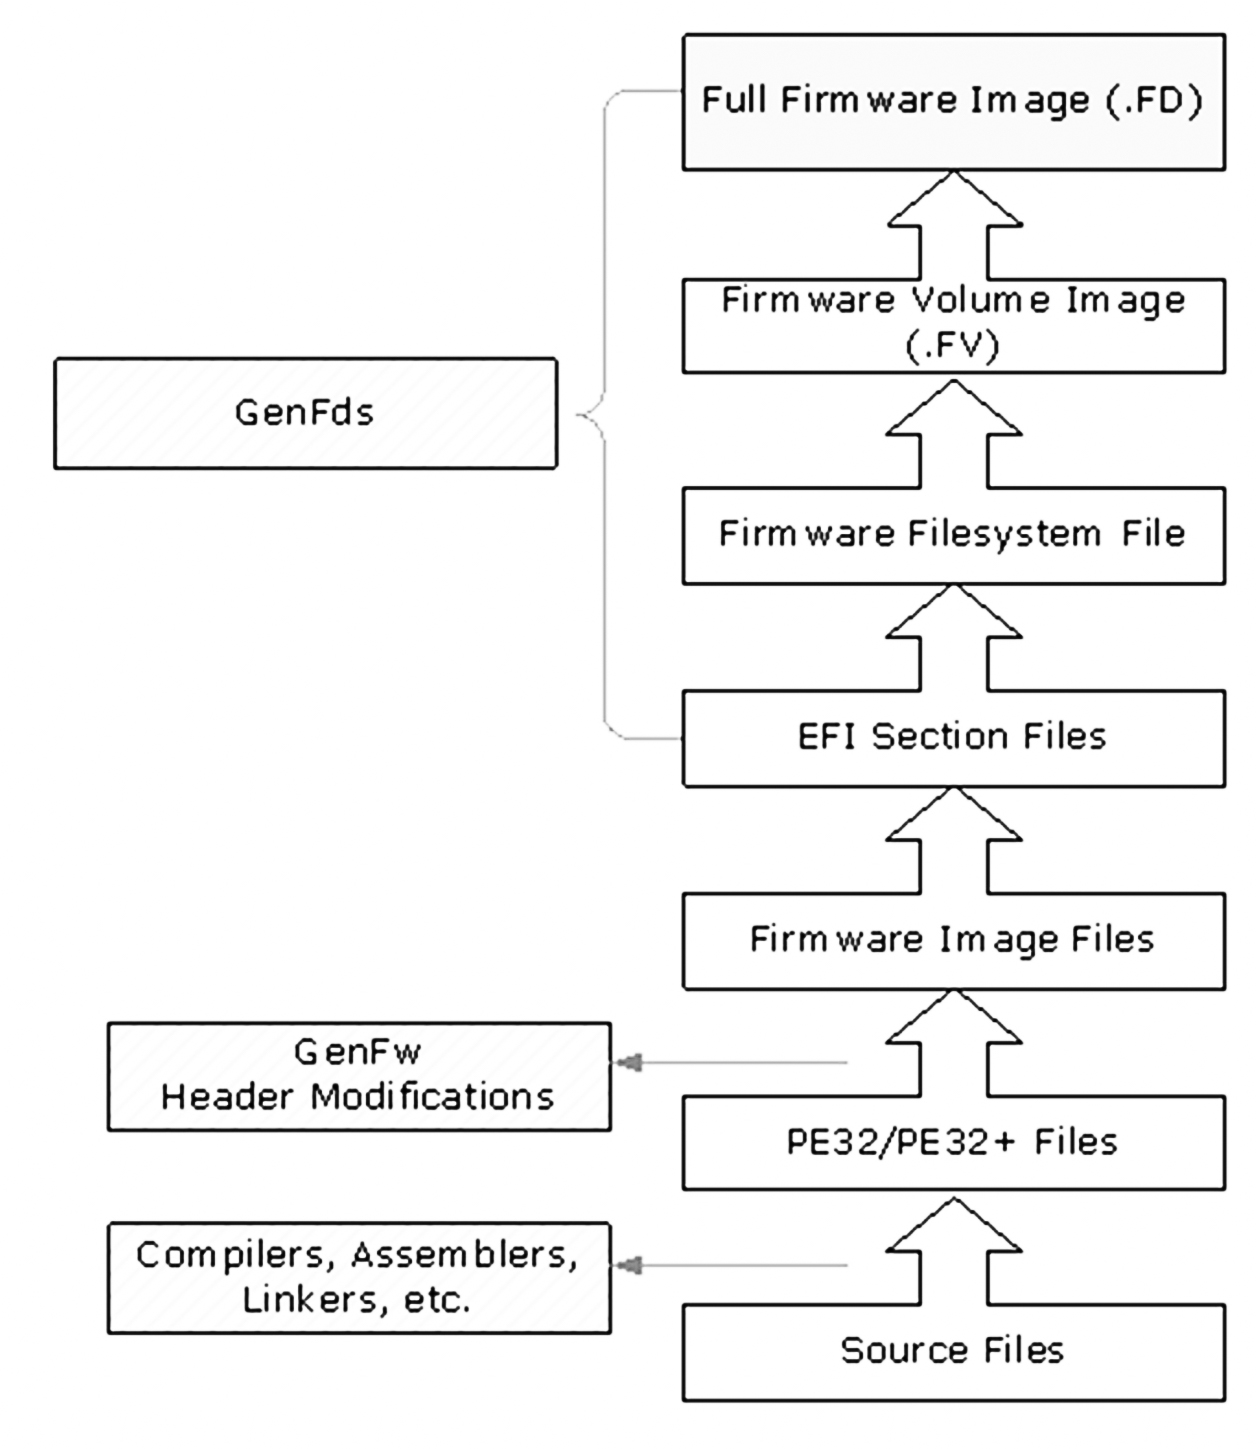
\includegraphics[width=0.9\linewidth]{design/uefi-pi-firmware-image-creation}
  \caption{UEFI/PI Firmware Image Creation}\label{fig:design-uefi-pi-firmware-image-creation}
\end{figure}
There are different layers of structure to a complete UEFI/PI firmware image. These layers are exemplified in Figure \ref{fig:design-uefi-pi-firmware-image-creation}. Every Shifts between layers means that a processing block that transforms or unites previously treated files into the another higher level. Also in Figure \ref{fig:design-uefi-pi-firmware-image-creation} portrayed the reference tools utilized that processes the files to transit them among the different layers. The layers are described in more emphasized manner in Section \ref{section-architecture}

Apart from constructing images that initialize the whole platform, the build process also sustains creation of standalone UEFI applications (such as OS Loaders) and ROM images having driver code. Figure \ref{fig:design-efi-application-creation} portrayed the reference implementation tools and creation processes for both the image type.

The closing feature that is backed by the EDK II build process is to packaged and distributed the founding of Binary Modules to be utilized by other governing body. Binary modules doesn't need to distribute the source code. This shall only allow vendors to publicize UEFI images \textbf{without releasing copyrighted source code}.

The process of packaging allows construction of an archive file having multiple binary files which can be either Firmware Image files or higher (FFS, EFI Section files, etc.). The build process would only allow insertion of such binary files in to the corresponding level of the build stages.
